\providecommand{\additionalOptionsForClass}{}
\documentclass[
  accentcolor=tud1c,	% Color theme for TUD corporate design
  colorbacktitle,		% Titlepage has colored background for title area
  inverttitle,			% Font color of title on titlepage is inverted
  \additionalOptionsForClass
  %german%,
  %twoside
]{tudexercise}

\parindent1em
%\parskip2ex

\usepackage[ngerman]{babel}
\usepackage[utf8]{inputenc}
\usepackage{listings}
\usepackage{booktabs}
\usepackage{amsmath}
\usepackage{algorithm2e}
\usepackage{hyperref}
\usepackage{xspace}
\usepackage{tabularx}
\usepackage{tikz}
\usepackage{cleveref}
\usepackage{numprint}
\usepackage{paralist}
\usepackage{verbatim}
\usepackage{tocloft} % for manipulating the table of contents

\usetikzlibrary{shapes}
\usetikzlibrary{calc}
\usetikzlibrary{arrows}
\usetikzlibrary{decorations}

\usepackage{pifont}
\newcommand{\cmark}{\ding{51}\xspace}%
\newcommand{\xmark}{\ding{55}\xspace}%

\usepackage{todonotes}
%\usepackage[disable]{todonotes} % Use this line to hide all todos

\definecolor{commentgreen}{RGB}{50,127,50}
\lstloadlanguages{C++,[gnu]make}
\lstset{language=C++}
\lstset{captionpos=b}
\lstset{tabsize=3}
\lstset{breaklines=true}
\lstset{basicstyle=\ttfamily}
\lstset{columns=flexible}
\lstset{keywordstyle=\color{purple}}
\lstset{stringstyle=\color{blue}}
\lstset{commentstyle=\color{commentgreen}}
\lstset{otherkeywords=\#include}
\lstset{showstringspaces=false}
\lstset{keepspaces=true}
\lstset{xleftmargin=1cm}
\lstset{literate=%
	{Ö}{{\"O}}1
	{Ä}{{\"A}}1
	{Ü}{{\"U}}1
	{ß}{{\ss}}2
	{ü}{{\"u}}1
	{ä}{{\"a}}1
	{ö}{{\"o}}1
	{'}{{\textquotesingle}}1
}

\lstnewenvironment{lstmake} %
{\lstset{language=[gnu]make}} %
{}


\newcommand{\superscript}[1]{\ensuremath{^{\textrm{#1}}}}
\newcommand{\subscript}[1]{\ensuremath{_{\textrm{#1}}}}

\newcommand{\setHeader}[1]{
\providecommand{\examheadertitle}{TODO: Titel einbinden}
\renewcommand{\examheadertitle}{#1}
\begin{examheader}
    \examheadertitle
\end{examheader}
}

\newcommand{\hints}[1]{
\paragraph*{Hinweise}
	\begin{itemize}
		\setlength{\itemsep}{0pt}
		#1
	\end{itemize}
}

\newcommand{\optional}{\xspace(optional)}
\newcommand{\experimental}{\xspace(experimentell)}

\usepackage{fancybox}
\newcommand{\optionaltextbox}{
	\bigskip
	\begin{center}
		\ovalbox{\parbox{0.98\textwidth}{Die Klausur kann ohne diese Aufgabe bestanden werden. Wir empfehlen aber sie trotzdem zu bearbeiten.}}
	\end{center}
}
\newcommand{\experimentaltextbox}{
	\bigskip
	\begin{center}
		\ovalbox{\parbox{0.98\textwidth}{Diese Aufgabe wurde neu erstellt und kann noch Fehler und Inkonsistenzen enthalten. Falls euch etwas derartiges auffällt sprecht uns bitte darauf an oder stellt es auf GitHub in den Issuetracker unter \url{https://github.com/Echtzeitsysteme/tud-cpp-exercises/issues}}}
	\end{center}
}

\newcommand{\enquote}[1]{\glqq#1\grqq\xspace}
\newcommand{\filename}[1]{\texttt{#1}}

\newcommand{\RK}[1]{\todo[]{\textbf{RK:} #1}}
\newcommand{\RKi}[1]{\todo[inline]{\textbf{RK:} #1}}

\newcommand{\ExercisePrefix}[1]{$[$#1$]$ \xspace}
\newcommand{\ExercisePrefixBasics}{\ExercisePrefix{G}}
\newcommand{\ExercisePrefixMemory}{\ExercisePrefix{S}}
\newcommand{\ExercisePrefixObjectOrientation}{\ExercisePrefix{O}}
\newcommand{\ExercisePrefixAdvanced}{\ExercisePrefix{F}}
\newcommand{\ExercisePrefixEmbeddedC}{\ExercisePrefix{C}}
\newcommand{\ExercisePrefixElevator}{\ExercisePrefix{A}}
\newcommand{\ExercisePrefixAdditionalInformation}{\ExercisePrefix{Z}}


\newcommand{\exday}{6}

\cppSetTitle

\begin{document}

\cppSetHeaderAndMakeTitle

\section{Implementation eines beliebigen Programms}
Nach Kennenlernen aller Ein- und Ausgabemöglichkeiten des Boards besteht die Aufgabe darin ein beliebiges Programm, zum Beispiel ein Spiel, zu implementieren.
Du hast hierbei die freie Wahl, die folgenden Vorschläge sollen nur als Anreiz dienen.
Um die Aufgabe leichter zu gestalten, empfiehlt es sich die beiliegende uc\_library zu verwenden (TODO siehe Dokumentation).

\section*{Vorschlag: Pong}
Zwei Gegner sollen je einen Balken (Rechteck) am linken oder rechten Rand des Spielfeldes mit den Schiebereglern steuern können, um einen Ball (ein Quadrat) im Spiel zu halten.
Erreicht der Ball den linken oder rechten Rand des Spielfelds, so bekommt der Spieler auf der anderen Seite einen Punkt und der Ball wird an seine Anfangsposition (die Mitte des Spielfelds) zurückversetzt.
Erreicht der Ball den oberen oder unteren Rand sowie einen der Balken der Spieler, so wird der Ball reflektiert - verlässt also niemals das Spielfeld.

Gewonnen hat der Spieler, der zuerst eine definierte Anzahl an Punkten erreicht.
Die aktuelle Punktzahl beider Spieler könnte auf der Siebensegmentanzeige ausgegeben werden.
\begin{center}
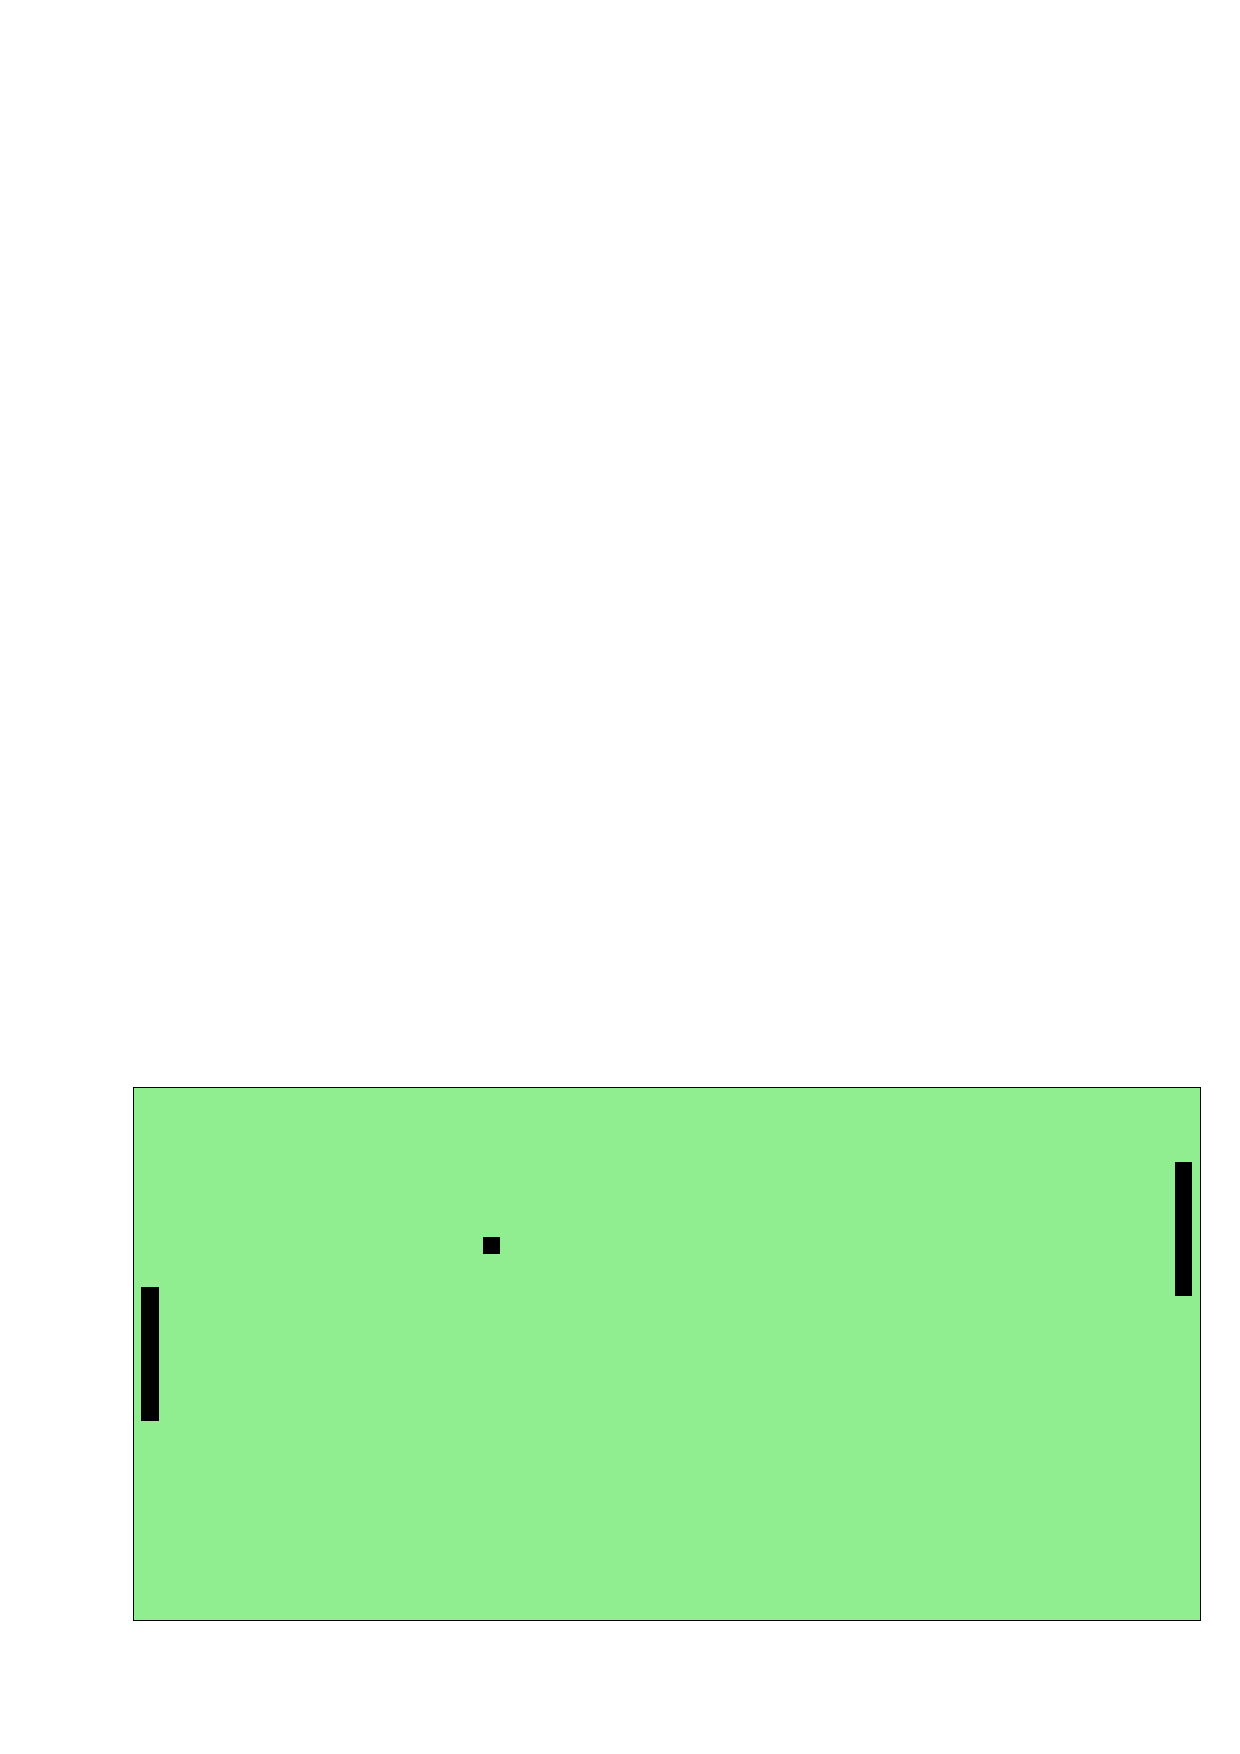
\includegraphics[scale=0.4]{figures/pong}
\end{center}



\section*{Vorschlag: Game of Life}
\glqq{}Game of Life\grqq{}\footnote{siehe auch \url{http://de.wikipedia.org/wiki/Conways_Spiel_des_Lebens}} besteht aus einem zweidimensionalen Spielfeld.
Jedes Feld steht für eine Zelle, die \textit{tot} (grün) oder \textit{lebendig} (schwarz) ist.
Jede Zelle hat acht Nachbarzellen, die ebenso tot oder lebendig sein können.
Zu Beginn gibt es eine vordefinierte Anfangsgeneration.

Durch festgelegte Regeln wird die nachfolgende Generation ermittelt:
\begin{itemize}
	\item Eine \textbf{lebende Zelle} \dots
	\begin{itemize}
		\item mit 1 oder 0 lebenden Nachbarn stirbt aus Einsamkeit.
		\item mit 4 oder mehr lebenden Nachbarn stirbt wegen Übervölkerung.
		\item mit 2 oder 3 lebenden Nachbarn bleibt am Leben.
	\end{itemize}
	\item Eine \textbf{tote Zelle} mit genau 3 lebenden Nachbarn wird in der nächsten Generation geboren werden, andernfalls bleibt sie tot.
\end{itemize}

Als Anfangsgeneration eignen sich zufällige Populationen oder eine der folgenden Figuren:

\begin{center}
	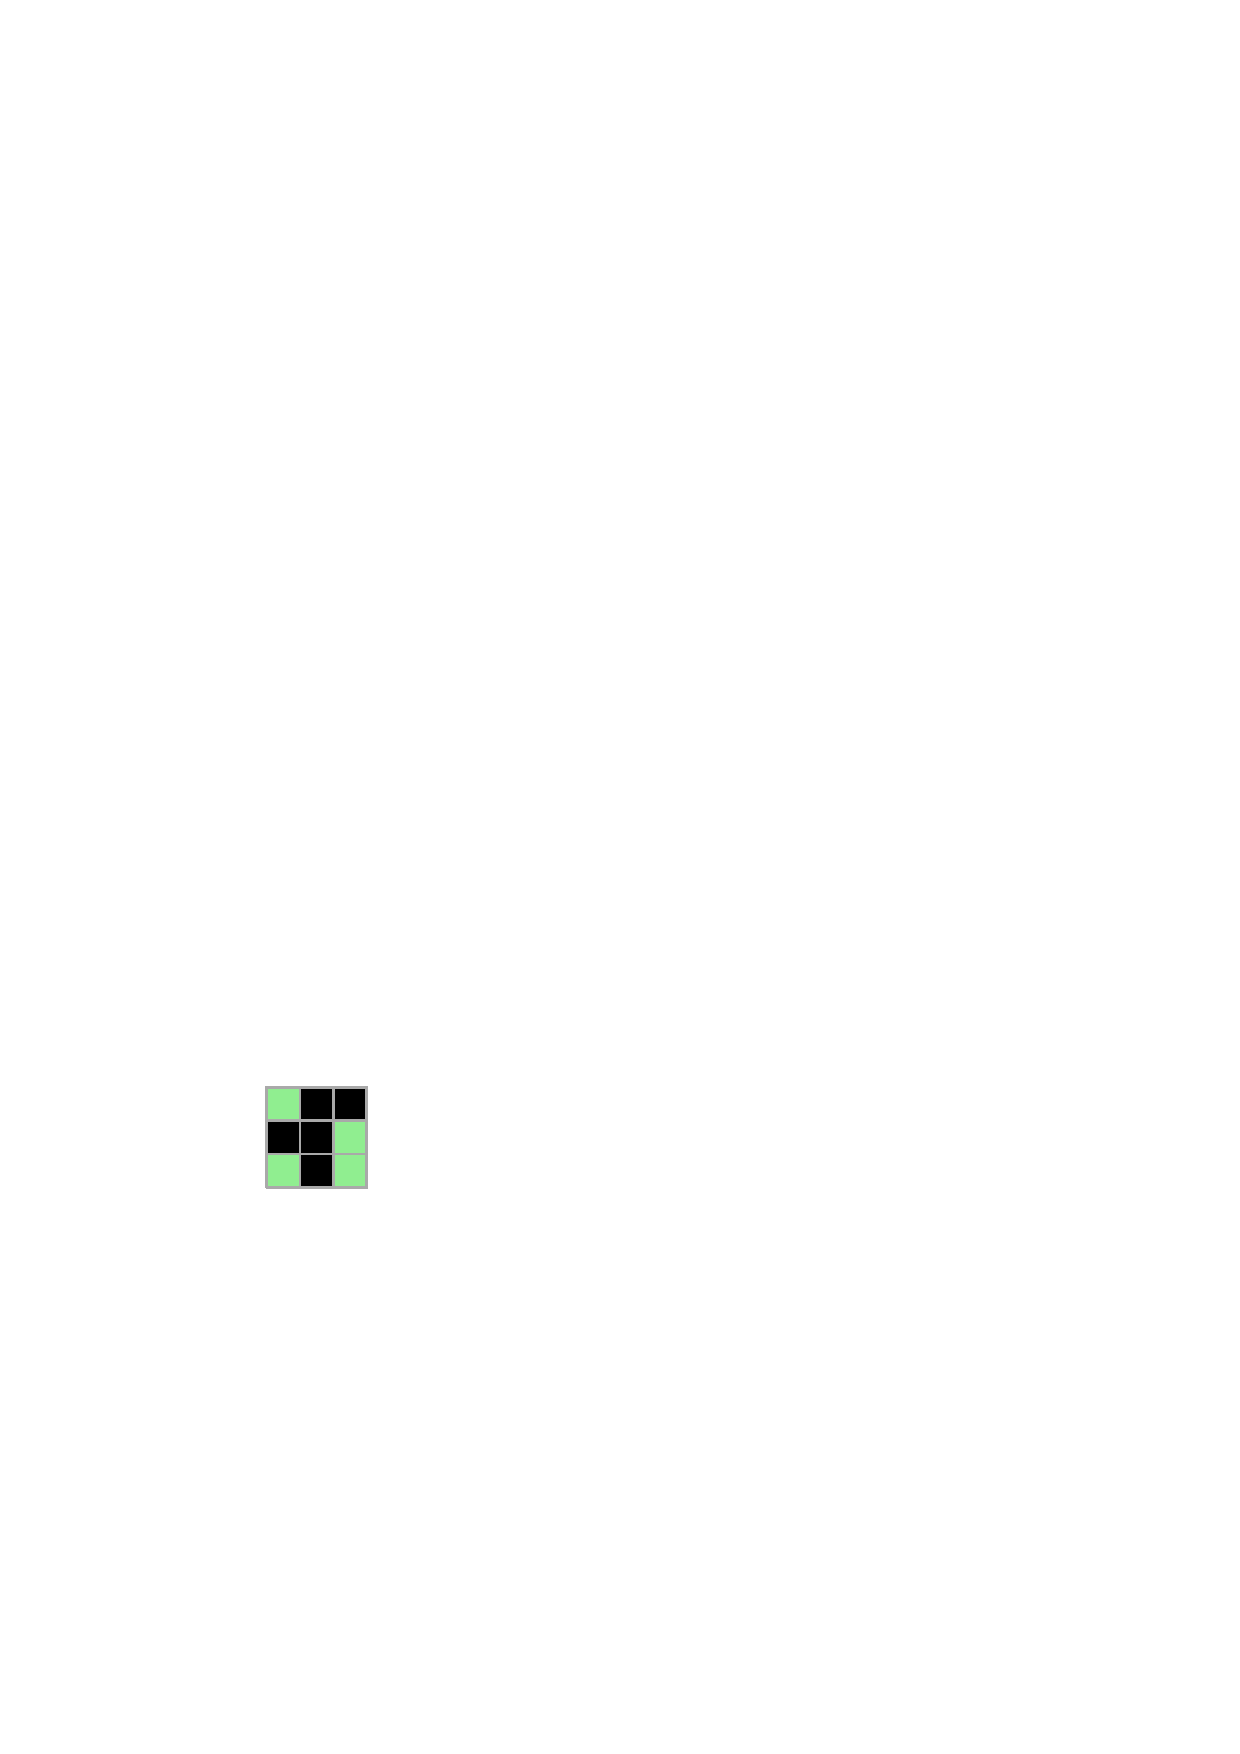
\includegraphics[scale=1]{figures/gol_init1}
	\hspace{5mm}
	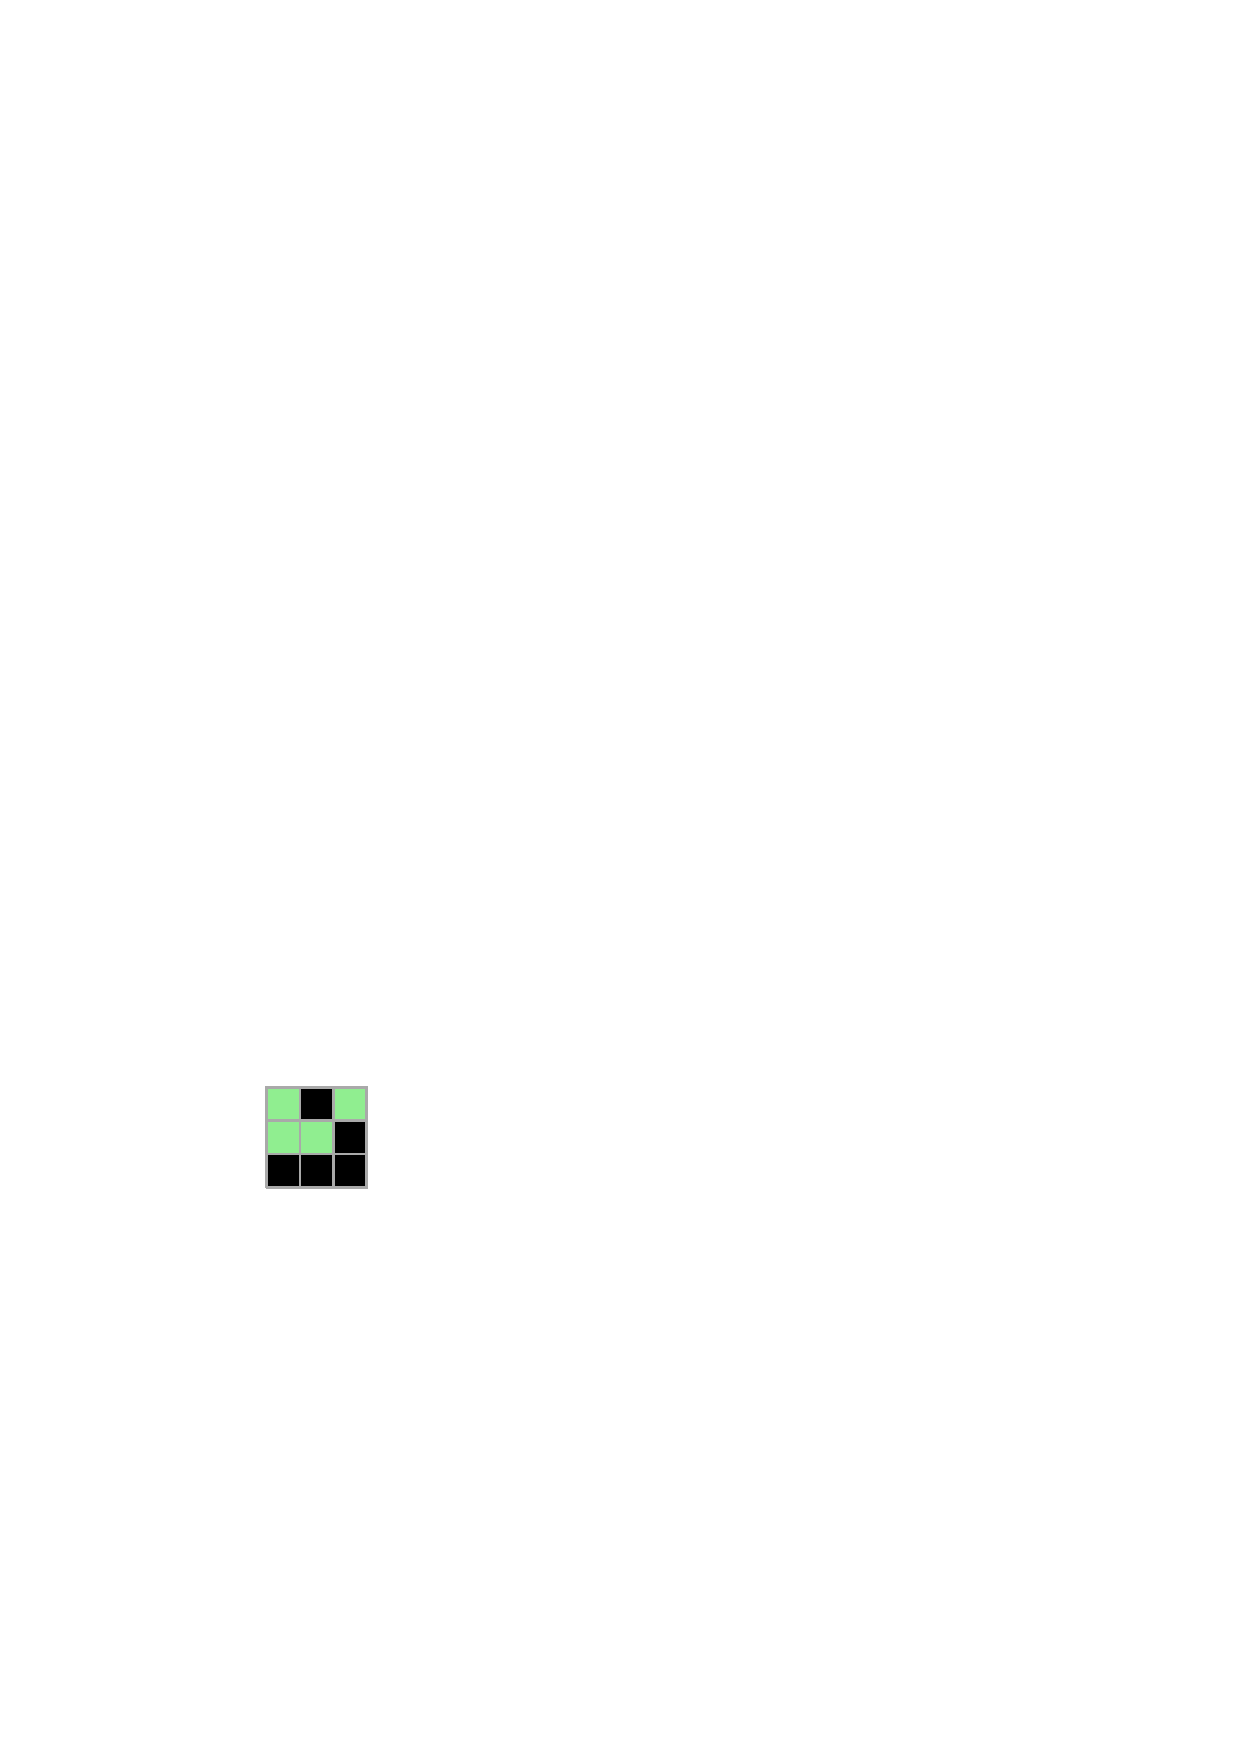
\includegraphics[scale=1]{figures/gol_init2}
	\hspace{5mm}
	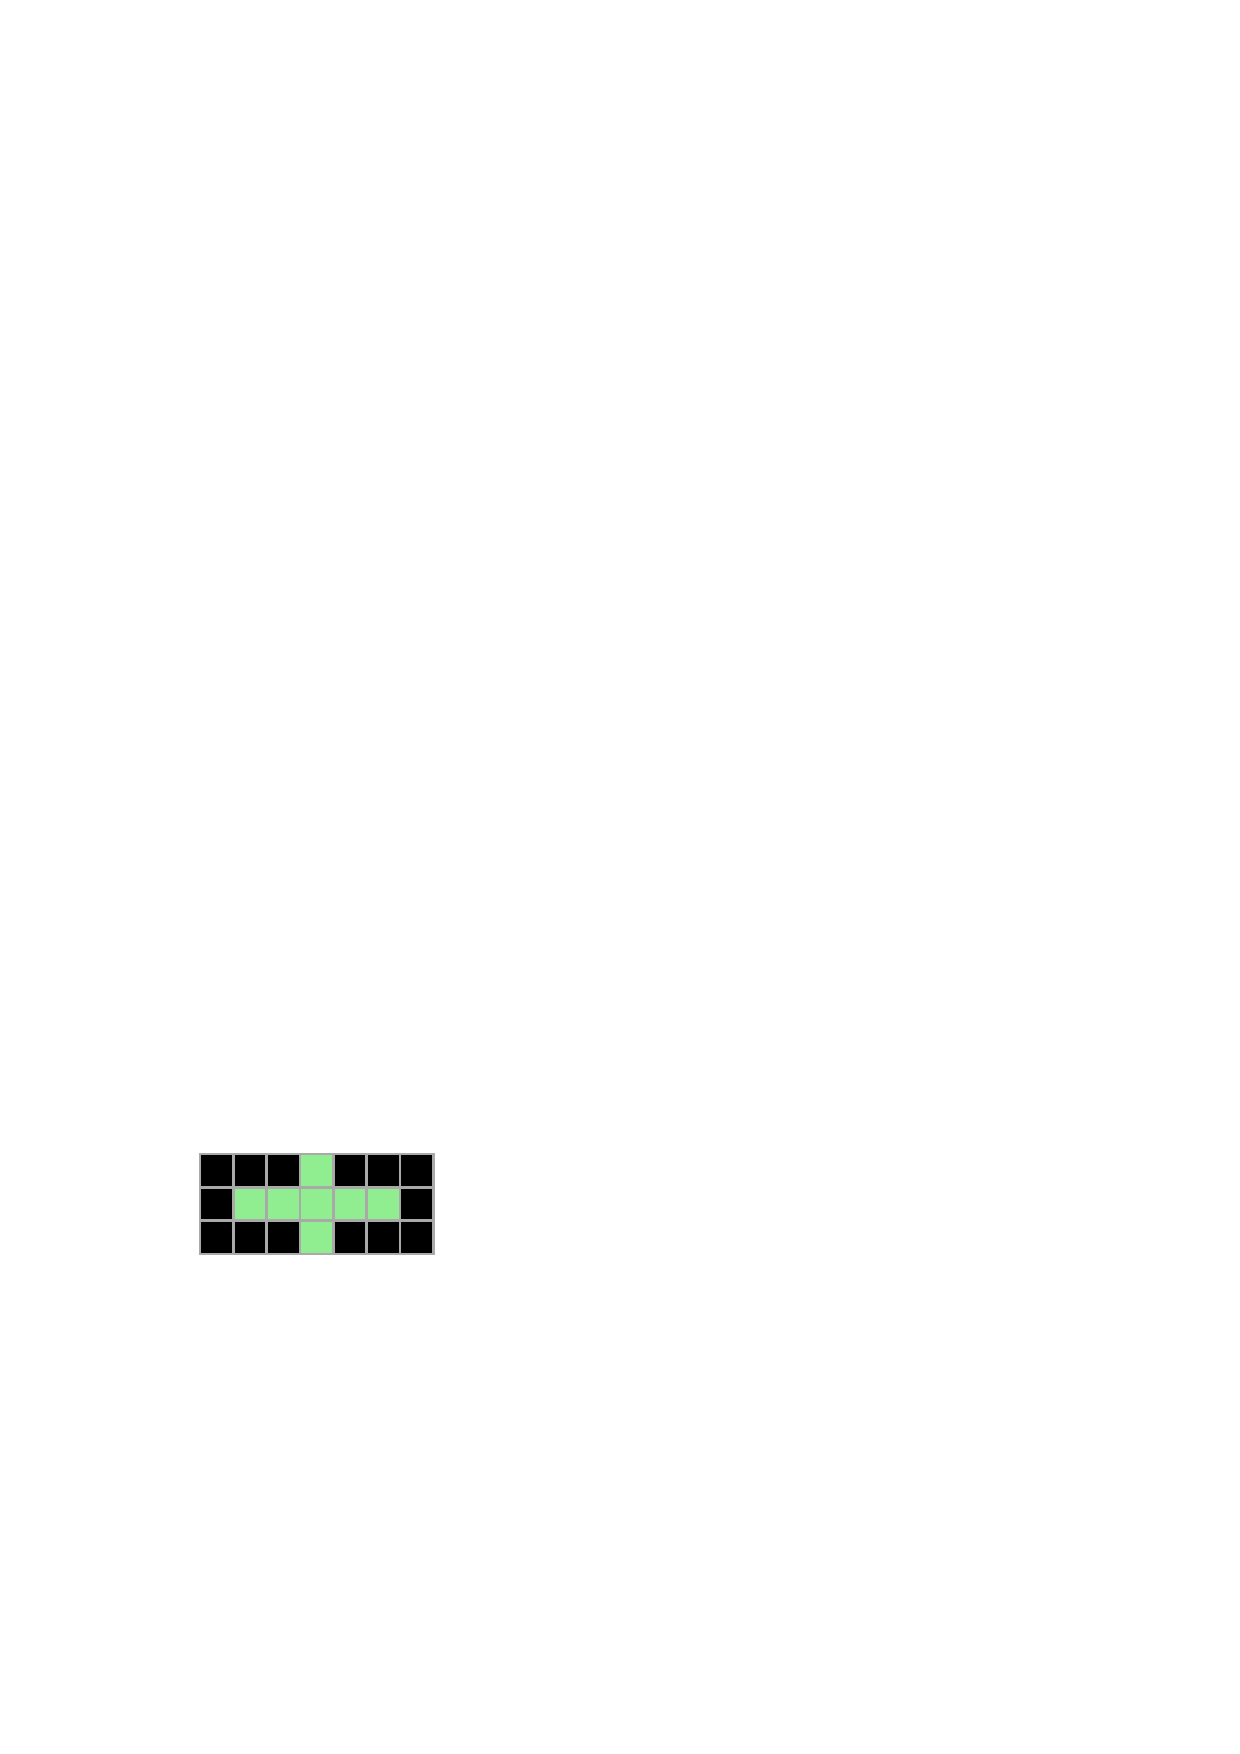
\includegraphics[scale=1]{figures/gol_init3}
\end{center}

\hints{
	\item Da das Spielfeld begrenzt ist soll es torusförmig aufgebaut werden (alles, was am unteren Rand des Spielfelds verschwindet, kommt oben wieder heraus -- das Gleiche gilt für den linken und rechten Rand). 
	\item Verwende als Spielfeld ein mehrdimensionales Array
	\item Ein weiteres mehrdimensionales Array bietet sich an, um die zukünftige Generation erzeugen zu können.
	\item Achte beim torusförmigen Feld unbedingt darauf, dass du nicht über die Grenzen des Spielfelds hinaus zugreifst!
}



\section*{Weitere Vorschläge}
\begin{minipage}{.45\textwidth}
    \begin{center}Asteroids\\\vspace{4ex} 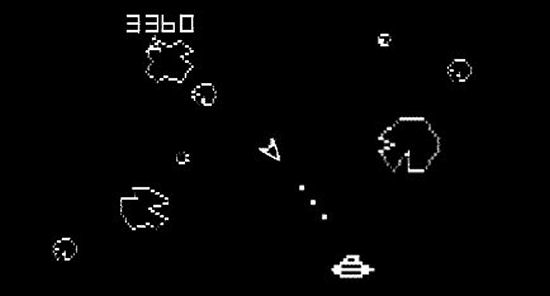
\includegraphics[width=.5\textwidth]{figures/img_asteroids.png}\end{center}
    \begin{center}Pacman\\\vspace{4ex}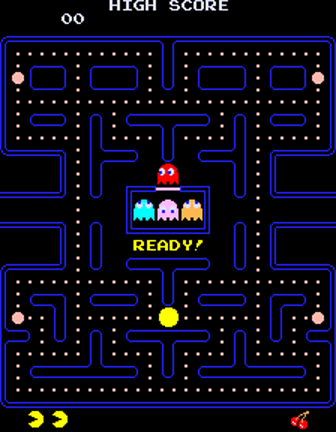
\includegraphics[width=.3\textwidth]{figures/img_pacman.png}\end{center}
    \begin{center}Labyrinth\\\vspace{4ex}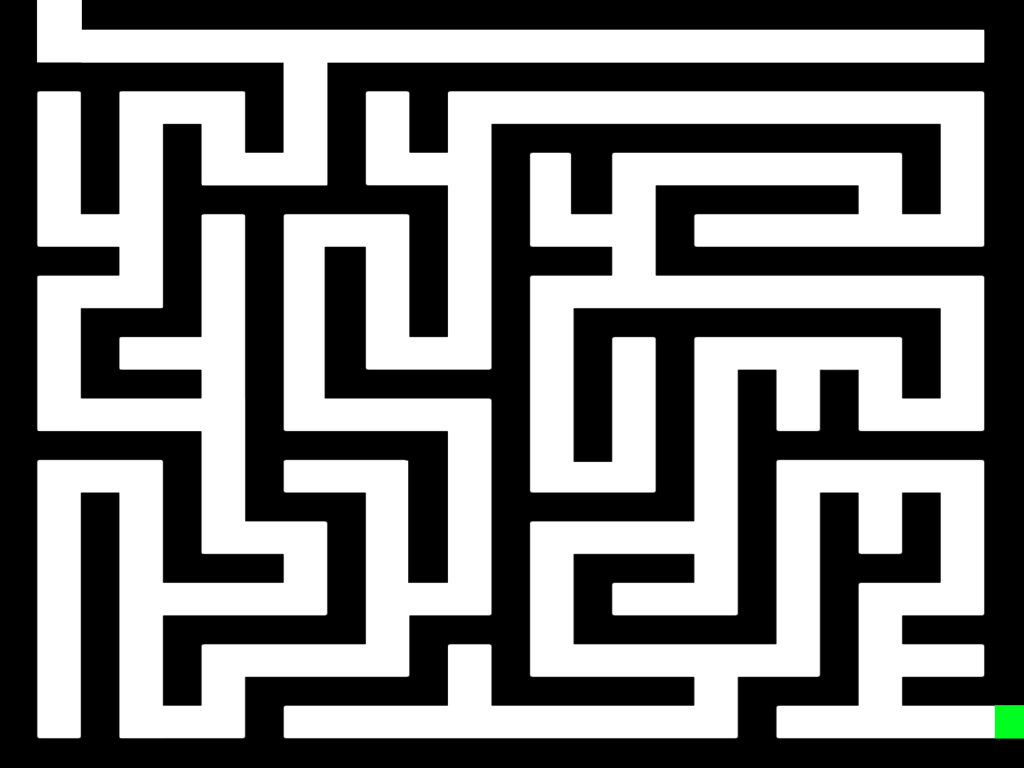
\includegraphics[width=.4\textwidth]{figures/img_maze.png}\end{center}
\end{minipage}
\begin{minipage}{.45\textwidth}
	\begin{center}Ausweichspiele à la Hugo\\\vspace{4ex}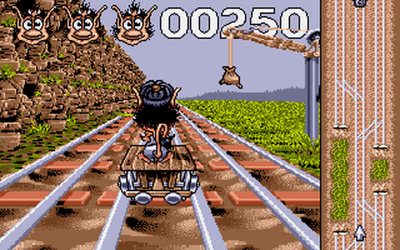
\includegraphics[width=.4\textwidth]{figures/img_hugo.png}\end{center}
	\begin{center}Moorhuhn\\\vspace{4ex}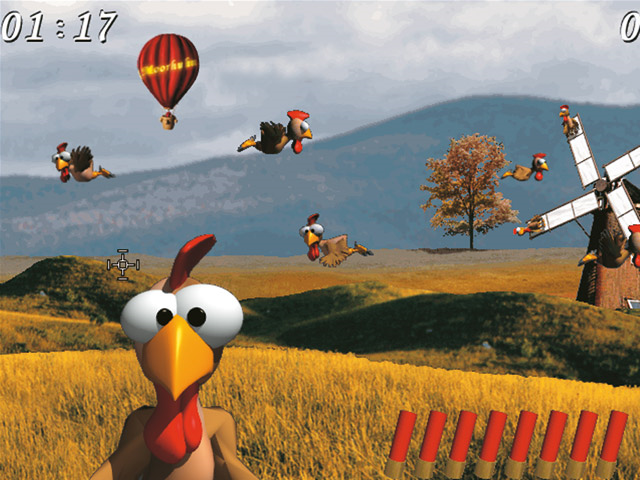
\includegraphics[width=.4\textwidth]{figures/img_moorhuhn.png}\end{center}
	\begin{center}Snake\\\vspace{4ex}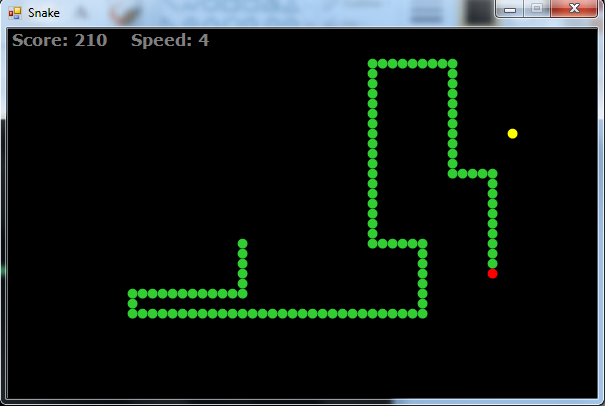
\includegraphics[width=.4\textwidth]{figures/img_snake.png}\end{center}
\end{minipage}


\end{document}
